\chapter{Maschinen}

\newpage

\section{DC-Maschine}

\begin{figure}[h!]
\centering
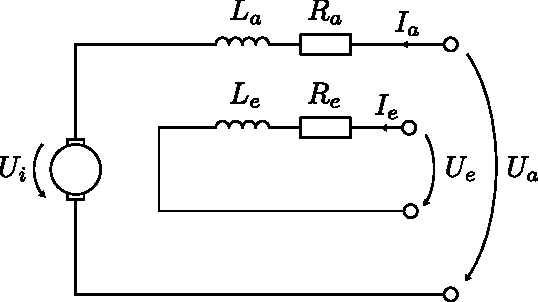
\includegraphics[scale=\schscale]{dc-motor.pdf}
\caption{Ersatzschaltbild einer DC-Maschine}
\label{sch:dc-maschine}
\end{figure}

\subsection{Verhalten und Kennlinie}

Eine DC- oder Gleichstrommaschine hat grundsätzlich drei Betriebszustände:
\begin{itemize}
	\item Ankerstellbereich
	\item Normbereich
	\item Feldschwächungsbereich
\end{itemize}

\begin{figure}[h!]
\centering
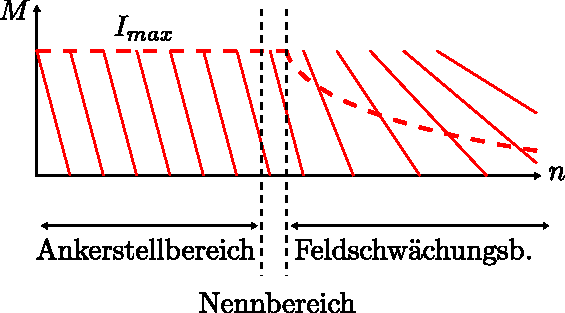
\includegraphics[scale=\schscale]{dc-motor-plot1.pdf}
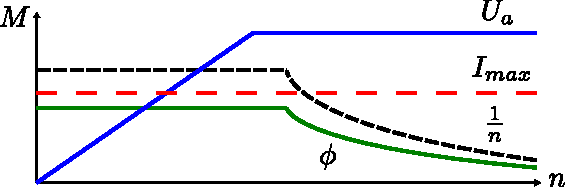
\includegraphics[scale=\schscale]{dc-motor-plot2.pdf}
\caption{Kennlinie einer DC-Maschine}
\label{fig:dc-motor-kennlinie}
\end{figure}

\noindent
Wichtig sind die foldengen Charakteristiken einer DC-Maschine:

\begin{itemize}
	\item Die Drehzahl ist proportional zur Spannung (falls unbelastet).
	\item Nimmt man der DC-Maschine Moment ab (d.h. belasten), so sinkt
		die Drehzahl linear ab bis hin zum maximalen Strom.
	\item	Blockiert man die Rotation (Reibung, Last) so überhitzt
		der Motor.
\end{itemize}

\subsection{Dynamischer Betrieb}
\[ \begin{array}{l}
U_a = U_i + (R_a \cdot I_a) + \left(L_a \cdot \frac{d I_a}{d t}\right) \\\\
U_e = (R_e \cdot I_e) + \left(L_e \cdot \frac{d I_e}{d t}\right) \\\\
U_i = c \cdot \Phi \cdot \omega_m \\\\
M_{el} = c \cdot \Phi \cdot I_a \\\\
M_{el} = M_{Welle} + M_{Reibung} + \left( J \cdot \frac{d \omega_m}{d t} \right) \\\\
\Phi = \frac{L_e}{N_e} \cdot I_e
\end{array} \]

\subsection{Stationärer Betrieb}
\[ \begin{array}{l}
U_a = U_i + (R_a \cdot I_a) \\\\
U_a = (c \cdot \phi \cdot \omega_m) + (R_a \cdot I_a) \\\\
\omega_m 
	= \frac{U_a - (R_a \cdot I_a)}{c \cdot \phi}
	= \frac{U_a}{c \cdot \phi} - \frac{R_a}{c \cdot \phi} \cdot I_a
	= \frac{U_a}{c \cdot \phi} - \frac{R_a}{(c \cdot \phi)^2} \cdot M
\end{array} \]

\newpage

\section{Serieerregte DC-Maschine}\label{sec:dc-motor-serie}

\begin{figure}[h!]
\centering
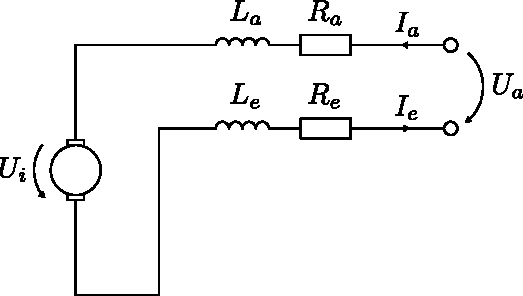
\includegraphics[scale=\schscale]{dc-motor-serie.pdf}
\caption{Ersatzschaltbild der serieerregten DC-Maschine}
\label{sch:dc-maschine-serie}
\end{figure}

\[ I_e = I_a \]
\[ \phi = \frac{L_e}{N_e} \cdot I_e = \frac{L_e}{N_e} \cdot I_a \]
\[ \omega_m = \frac{U_a - (R_a + R_e) \cdot I_a}{c \cdot \frac{L_e}{N_e} \cdot I_a} \]
\[ M_{el} = c \cdot \frac{L_e}{N_e} \cdot I_a^2 \]
\[ U_a = (R_a + R_e) \cdot I_{e,a} + U_i + (L_a + L_e) \cdot \frac{d I}{d t} \]
\[ U_i = c \cdot \frac{L_e}{N_e} \cdot I \cdot \omega_m \]
\[ \omega_m = \frac{U_a - (R_a + R_e) \cdot I}{c \cdot \frac{L_e}{N_e} \cdot I} \]
\[ \omega_m \approx \frac{U_a}{c \cdot \frac{L_e}{N_e} \cdot \sqrt{\frac{N_e \cdot M}{c \cdot L_e}}} 
	= \frac{U_a}{\sqrt{c \cdot \frac{L_e}{N_e}}} \cdot M \]

\newpage

\section{Universalmotor}

Diese elektrische Maschine kann sowohl mit DC als auch mit AC betrieben
werden ohne Veränderungen vorzunehmen, deshalb werden die Doppelnamen 
\textit{Serieerregte Gleichstrommaschine} und 
\textit{Einphasen-Reihenschluss"-motor} benutzt.

Wird die Maschine mit DC betrieben, so gelten die Formeln aus dem Kapitel
\ref{sec:dc-motor-serie}. Wird die Maschine mit AC betrieben, so müssen die
folgenden Formeln benutzt werden.

\[ \underline{U} = (R_a + R_e) \cdot \underline{I} + j \cdot \omega \cdot (L_a + L_e) \cdot \underline{I} + \underline{U_i} \]
\[ \underline{U_i} = c \cdot \phi \cdot \omega_m = c_1 \cdot \underline{I} \cdot \omega_m \]
\[ |\underline{U^2}| = (|U_i| + R \cdot |\underline{I}|)^2 + (\omega \cdot L \cdot |\underline{I}|)^2, \quad U_i = c_1 \cdot |\underline{I}| \cdot \omega_m \]

\begin{figure}[h!]
\centering
\caption{Zeigerdiagramm des Universalmotors bei AC-Betrieb}
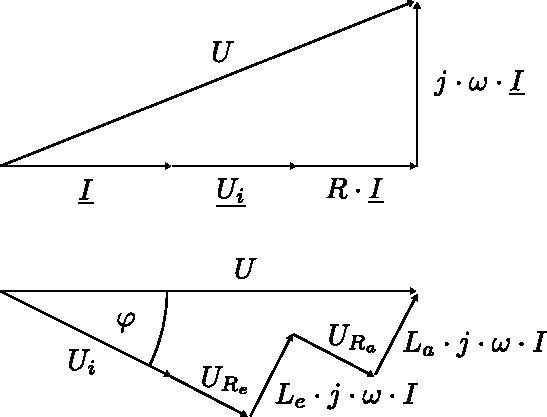
\includegraphics[scale=\schscale]{dc-motor-serie-plot1.pdf}
\label{fig:universalmotor-zeiger}
\end{figure}













































